\chapter{Design}
The fourth chapter, \textit{Design}, presents the results of the user interface design, the created algorithm to determine the parking position of a user's car and the applied machine learning workflow. The first section, \textit{User Interface}, presents the four iterations of the user interface and explains the design decisions of the final user interface design. The second section, \textit{Determine the Parking Position}, describes the algorithm used to determine the parking position of an user's car based on their spatial trajectory. The third section, \textit{Transportation Mode Classification of Spatial Trajectories}, describes the process conducted to train a machine learning model that classifies the transportation mode of a spatial trajectory.

\section{User Interface}
The first section, \textit{User Interface}, presents the designed user interface. First, the four iterations and the changes between them are described. Second, the final user interface design is discussed by considering usability heuristics by Nielsen and Apple.

\subsection{Iterations}
In the first part, \textit{Iterations}, the different iterations of the user interface and their related Think-Aloud protocol results are presented. The full user interface of each iteration can be seen in Appendix \ref{appendix:userInterface}.

\paragraph{First Iteration}

The first iteration consists of five views. The application starts in the ''MapView - Loading'' view (cp. Figure \ref{fig:i1-mv-loading}). The view shows a map on which the location of the user is marked. At the top of the page a string indicates the current loading state of the system.

If the application fails to determine the parking position, a pop-up menu is shown (cp. Figure \ref{fig:i1-mv-error}) which notifies the user about the problem and explains the cause of the failure. 


\begin{figure}[h]
  \centering
  \begin{minipage}[b]{0.45\textwidth}
    \centering
    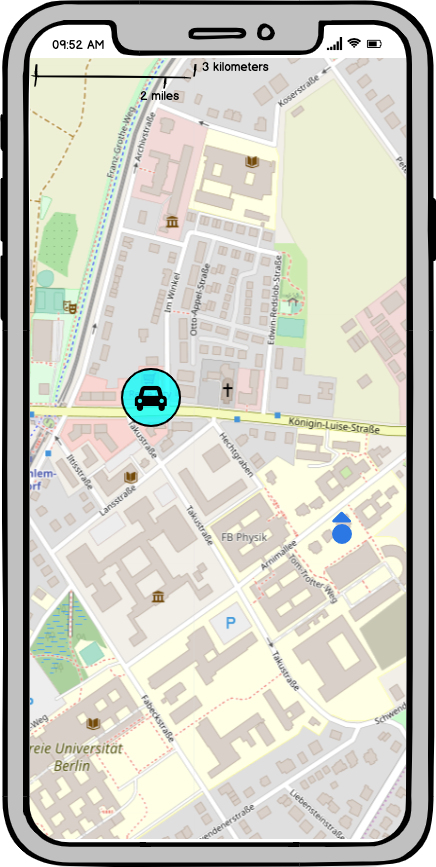
\includegraphics[width=0.75\textwidth]{images/UI/Iteration1-MapView-ParkingPositionDetermined.png}
  \end{minipage}
  \hfill
  \begin{minipage}[b]{0.45\textwidth}
    \centering
    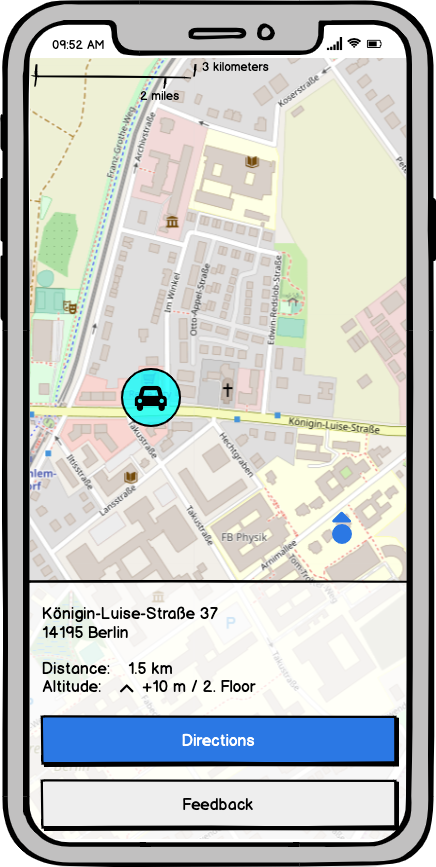
\includegraphics[width=0.75\textwidth]{images/UI/Iteration2-MapView-ParkingPositionDetermined.png}
  \end{minipage}
  \caption{Iteration 1: MapView - Parking Position Determined (left), Iteration 2: MapView - Parking Position Determined (right)}
  \label{fig:i1-i2}
\end{figure}



On successful determination of the parking position, the view ''MapView - Determined Parking Postition'' (cp. Figure \ref{fig:i1-i2}) is shown. It shows a map with the user's location and the determined position of the user's car. The label of the user's car is clickable and opens ''MapView - Details''. 

''MapView - Details'' (cp. Figure \ref{fig:i1-mv-details}) presents more details about the determined parking position. It presents the address where the car is parked, the distance to the user's car, the altitude difference between the user and the user's car and the floor of the parked car. Two buttons are presented: One button opens a third party navigation software to navigate to the determined location and the other button initiates the reporting of the accuracy of the determined parking position by opening the ''Feedback'' view.

The ''Feedback'' (cp Figure \ref{fig:i1-feedback}) view presents the user instructions to report the accuracy of the determined parking position, the transmitted information and a button to report the information. When the button is clicked, the information is sent and the application returns to the previous view, ''MapView - Details''. The user can also go back to the previous screen without sending any information by using the ''Back'' button.


The Think-Aloud protocol shows two key findings. First, in the view ''MapView - Parking Position Determined'', the user does not understand that the car icon is clickable. Second, the user expects to be able to give feedback in text form in the ''Feedback'' view.

\paragraph{Second Iteration}

In the second iteration of the user interface, the two problems of the first iteration are improved. The views ''MapView - Details'' and ''MapView - Parking Position Determined'' are merged. This change allows the user to see all details of the determined parking position directly. As the main view, ''MapView - Parking Position Determined'' (cp. Figure \ref{fig:i1-i2}), now shows a partly transparent white box. This element is also added to the ''MapView - Loading'' view to keep the user interface consistent. It contains a button to initiate the determination of the car. 
In the new ''MapView - Parking Position Determined'' view, the call to action to give feedback is rephrased to ''Send Accuracy'' to better represent the kind of feedback that can be given. The headline of the ''Feedback'' (cp. Figure \ref{fig:i2-feedback}) view is changed accordingly. A pop-up window is introduced in the ''Feedback'' view to confirm the successful sending of the accuracy.

The Think-Aloud protocol of the second iteration shows three key findings. First, the altitude in the view ''MapView - Parking Position Determined'' is understood as the total altitude of the car, but it shows the relative altitude of the car compared to the current altitude of the user. Second, the user is unsure if the presented address is the address of the location of the car, but assumes so. Third, the user does not notice in the ''Feedback'' view that the accuracy is supposed to be reported at the actual parking position of the car.


\begin{figure}[h]
  \centering
  \begin{minipage}[b]{0.45\textwidth}
    \centering
    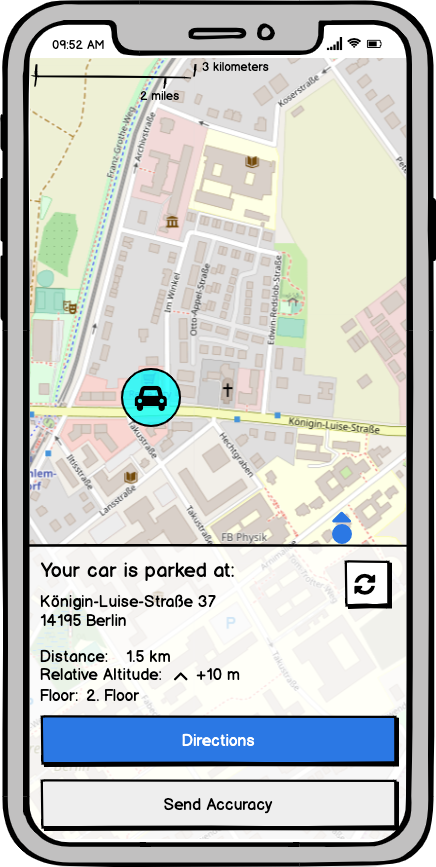
\includegraphics[width=0.75\textwidth]{images/UI/Iteration3-MapView-ParkingPositionDetermined.png}
  \end{minipage}
  \hfill
  \begin{minipage}[b]{0.45\textwidth}
    \centering
    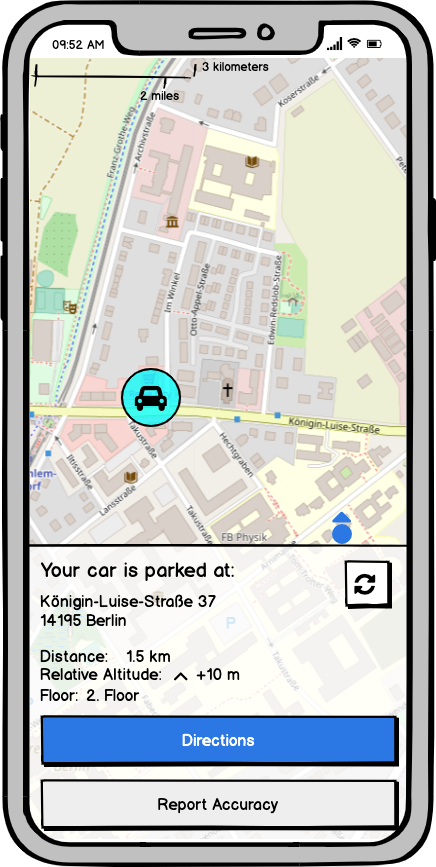
\includegraphics[width=0.75\textwidth]{images/UI/Iteration4-MapView-ParkingPositionDetermined.png}
  \end{minipage}
  \caption{Iteration 3 - MapView - Parking Position Determined (left), Iteration 4 - MapView - Parking Position Determined (right)}
  \label{fig:i3-i4}
\end{figure}

\paragraph{Third Iteration}

The third iteration improves on the three obstacles of the previous iteration. 
First, in the view ''MapView - Parking Position Determined'' (cp. Figure \ref{fig:i3-i4}) the altitude information is split  into two rows. The row ''Relative Altitude'' shows the relative altitude between the user's location and the car's location. The row ''Floor'' shows the floor of the determined parking location, if the data is available. Second, the headline ''Your car is parked at:'' is added to the view ''MapView - Parking Position Determined'' to clarify that the presented information is about the determined parking position. Third, a pop-up window is introduced in the view ''Feedback'' (cp. Figure \ref{fig:i3-feedback-con}) to ensure the user is actually at the location of the parked car. 

The Think-Aloud protocol shows one key finding. The call to action on the ''MapView - Parking Position Determined'' view to report the accuracy of the determined parking position is still not clear. The user is confused because the wording is unusual for giving feedback to improve an application.

\paragraph{Fourth Iteration}

To make the call to action to report the accuracy on the view ''MapView - Parking Position Determined'' (cp. Figure\ref{fig:i3-i4}) more clear, it is rephrased to ''Report Accuracy''. The headline of the view ''Feedback'' (cp. Figure \ref{fig:i4-feedback}) is updated accordingly. To the view ''MapView - Parking Position Determined'' a button is added to enable the user to refresh the determined parking position. 

\subsection{Final User Interface}

The second part, \textit{Final User Interface}, discusses the final user interface design. The different views are presented and design decisions argued based on the user interface heuristics by Apple Inc. and Nielsen. \cite{nielsen1994usability} \cite{apple:interfaceguidliines}

\paragraph{MapView - Loading}

\begin{figure}[h]
    \centering
    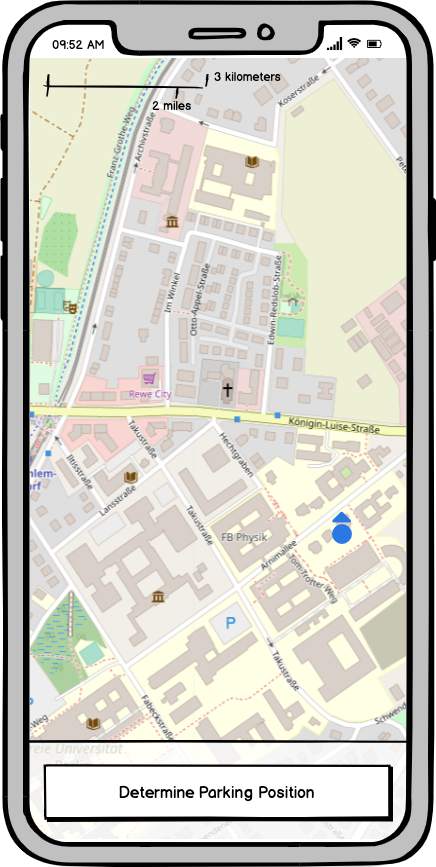
\includegraphics[width=0.4\textwidth]{images/UI/Iteration4-MapView-Loading.png}
    \caption{MapView - Loading}
    \label{fig:mv-loading}
\end{figure}

The application starts in the ''MapView - Loading'' view, shown in Figure \ref{fig:mv-loading}. The view consist of a map and a button to initiate the determination of the parking position of the user's car. The shown map supports the user to orientate themselves in their current environment by presenting their location on the map. Thus, the second heuristic from Nielsen, ''Match between system and the real world'', is implemented. The map is interactive and can be zoomed, moved and rotated. The button to determine the parking position of the user's car is placed on top of a white and partly transparent box to ensure a sufficient contrast between the map and the button. The design fulfils Apples design guidelines for MapKit\footnote{Apple Map Kit: \url{https://developer.apple.com/documentation/mapkit}, (online: last accessed October 19, 2019) }. The basic design of a map with a white, partly transparent box is used for all of the applications views, except the ''Feedback'' view, to keep the design simple and consistent, according to Nielsens fourth and eight heuristics. \cite{nielsen1994usability} \cite{apple:interfaceguidliines}

\newpage

\paragraph{MapView - Error}

\begin{figure}[h]
    \centering
    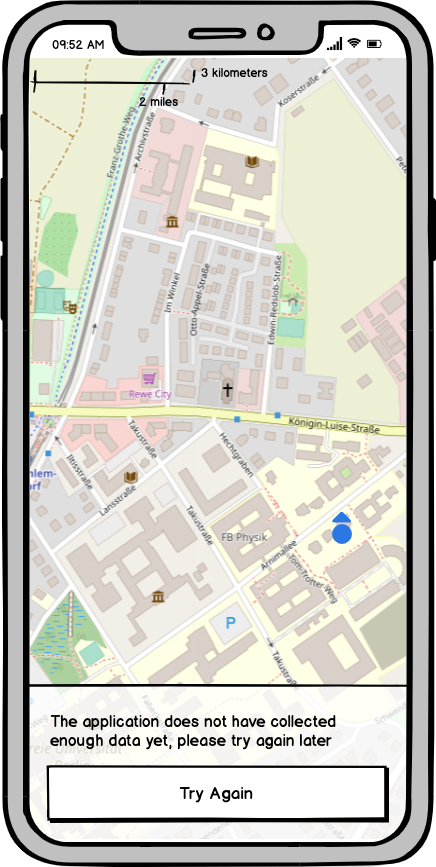
\includegraphics[width=0.4\textwidth]{images/UI/Iteration4-MapView-Error.png}
    \caption{MapView - Error}
    \label{fig:mv-error}
\end{figure}

If the application fails to determine the parking position of the user's car, it shows the view ''MapView - Error'', shown in Figure \ref{fig:mv-error}. The view shows a map with the user's location. On the bottom, an error message is printed on top of a white, partly transparent box. The error message explains in an understandable way for the user, why the application failed to determine the parking position. Below the error text, a button is shown. When pressed, the application tries to determine the parking position again. With the understandable error message and the promoted button to retry, the application confirms to Nielsens ninth heuristic, ''Help users recognize, diagnose, and recover from errors''. \cite{nielsen1994usability}

\paragraph{MapView - Parking Position Determined}

\begin{figure}[h]
    \centering
    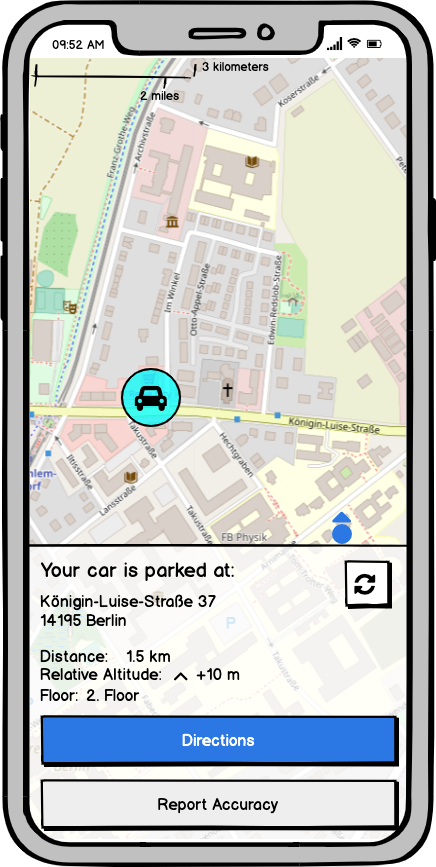
\includegraphics[width=0.4\textwidth]{images/UI/Iteration4-MapView-ParkingPositionDetermined.png}
    \caption{MapView - Parking Position Determined}
    \label{fig:mv-parking}
\end{figure}

The view ''MapView - Parking Position Determined'', shown in Figure \ref{fig:mv-parking}, is the main view of the application. It is shown when the application determined successfully the parking position of the user's car. A map and a partly transparent white box are shown. On the map, the user's current location and the position of the user's car are marked. The user's location is presented with a blue point. The location of the car is marked with a stylised car surrounded by a transparent circle. The car icon is on the exact location, the application determined as the parking position and the circle represents the accuracy of the determined parking location. The map view is chosen to match the system to the surroundings of the user. On the bottom of the screen, detailed information of the determined parking location are presented. The address, the distance to the current location, the relative altitude and the floor in which the car is parked are shown. Above the details, the headline ''Your car is parked at'' clearly identifies the listed information as related to the user's car. Three buttons are shown. The first button, in the upper right corner of the white box, refreshes the determined parking location. The second button, labelled ''Directions'', opens a third party navigation software to navigate to the determined location. Because navigation apps, such as Apple Maps and Google Maps, use the color blue to indicate a button which starts a navigation, the color blue is also chosen for the ''Directions'' button. The third button, labeled ''Report Accuracy'', initiates the process of reporting the accuracy of the determined parking location. The refresh button and the ''Report Accuracy'' button are both colored white to not draw extra attention to them. Most users should not need to use them on a regular base. \cite{nielsen1994usability}

\paragraph{Feedback}

\begin{figure}[h]
  \centering
  \begin{minipage}[b]{0.49\textwidth}
    \centering
    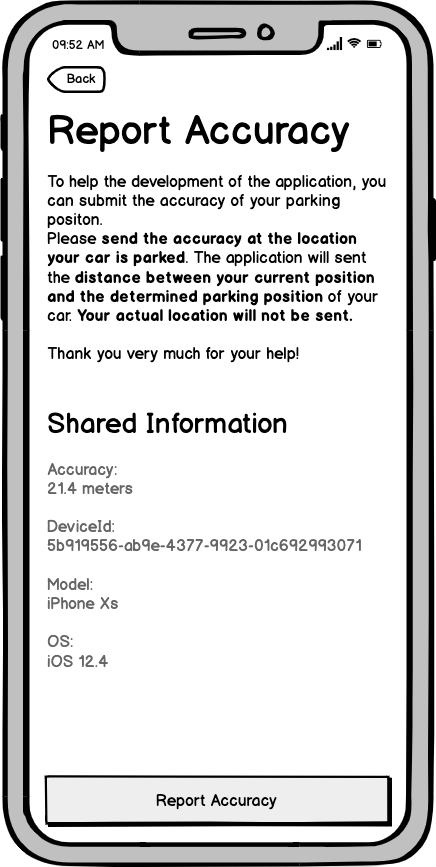
\includegraphics[width=0.6\textwidth]{images/UI/Iteration4-Feedback.png}
    \caption{Feedback}
    \label{fig:feedback}
  \end{minipage}
  \hfill
  \begin{minipage}[b]{0.49\textwidth}
    \centering
    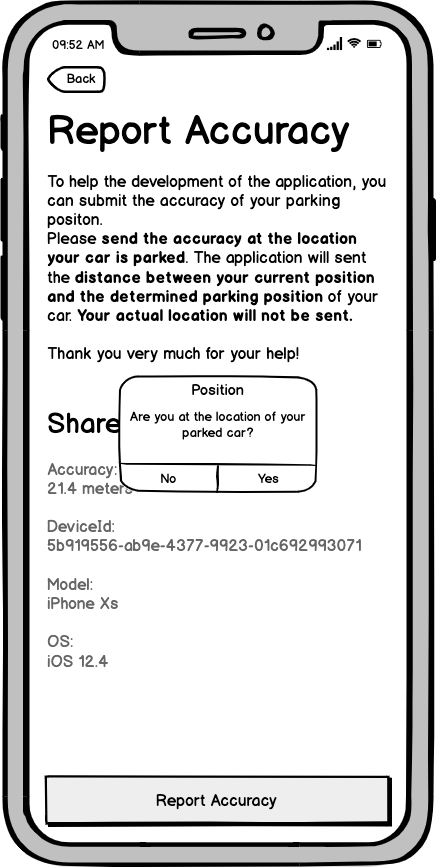
\includegraphics[width=0.6\textwidth]{images/UI/Iteration4-Feedback-Confirmation.png}
    \caption{Feedback - Confirmation}
    \label{fig:feedback-con}
  \end{minipage}
  
\end{figure}

The view ''Feedback'', shown in Figure \ref{fig:feedback}, enables the user to report the accuracy of the determined parking location. This functionality enables the quantitative evaluation of the systems accuracy. The text in the upper half of the screen explains how to report the accuracy and what kind of data is transmitted. A complete list of the transmitted data is shown in the bottom half. The ''Back'' button in the upper left corner navigates the system back to the view ''MapView - Parking Position Determined'' without transmitting any data. The button on the bottom, labelled ''Report Accuracy'', brings up a pop-up window in which the user is asked, if they are at the location of the parked car (cp. Figure \ref{fig:feedback-con}). The instructions in the explaining text are often skimmed by the users, thus this second check is necessary to keep the reported accuracy usable. If the user confirms their location, the data is send and a confirmation is shown (cf. Figure \ref{fig:feedback-succ}). The view changes back to the ''MapView - Parking Position Determined'' view. If the user does not confirm their location, a pop up is shown (cp. Figure \ref{fig:feedback-fail}) which asks the user to report the accuracy at the location of their parked car. The ''Back'' button enables the user to be in control if they want to share any information. The confirmation dialog prevents the user from accidental sending the accuracy at the wrong location. Thus, the view fulfills the third and fifth heuristic by Nielsen. \cite{nielsen1994usability} \newpage

\begin{figure}[h]
  \centering
  \hfill
  \begin{minipage}[b]{0.49\textwidth}
    \centering
    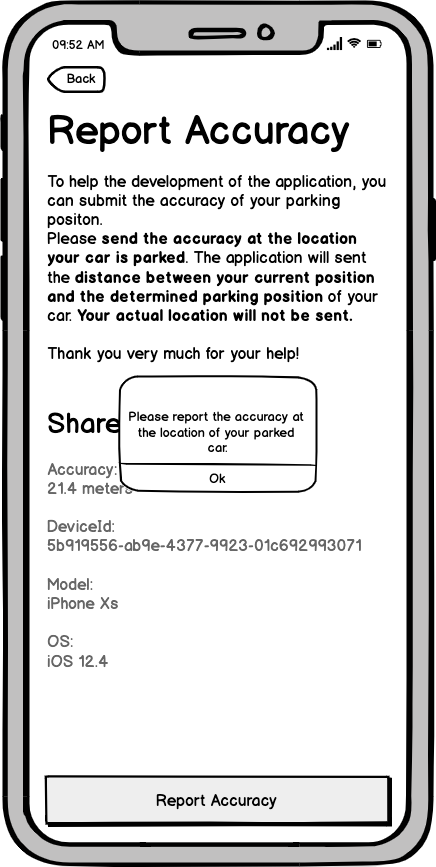
\includegraphics[width=0.6\textwidth]{images/UI/Iteration4-Feedback-Failure.png}
    \caption{Feedback - Failure}
    \label{fig:feedback-fail}
  \end{minipage}
  \hfill
  \begin{minipage}[b]{0.49\textwidth}
    \centering
    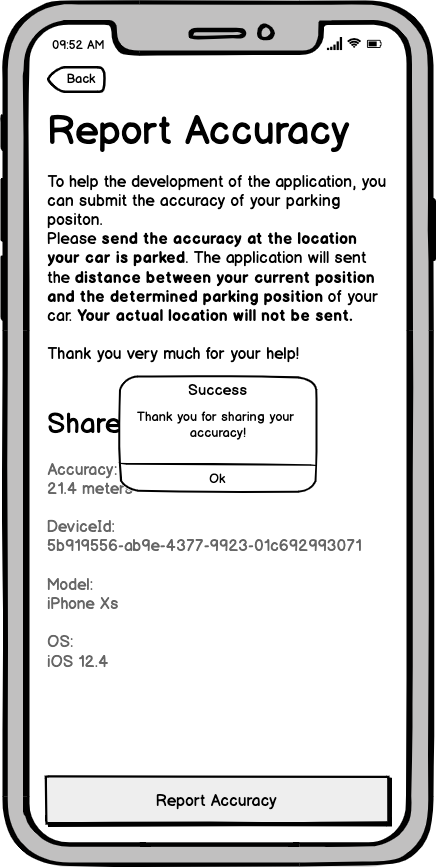
\includegraphics[width=0.6\textwidth]{images/UI/Iteration4-Feedback-Success.png}
    \caption{Feedback - Success}
    \label{fig:feedback-succ}
  \end{minipage}
\end{figure}

\section{Determining the Parking Position of a Car}
The algorithm to determine the parking position of a user's car (Source Code \ref{code:DetParkPos}) uses the heuristic that the user's car is parked where the user last traveled by car. To determine this location, the algorithm first removes the noise from the user's trajectory. The cleaned trajectory is segmented into individual trips based on the stay points of the trajectory. The trips are sorted from newest to oldest and examined for parking position candidates. The most recent of these candidates is returned as the determined parking position.

The algorithms applied in the parking position determination, namely the algorithms for noise removal, stay point detection, trip detection and parking position candidate detection are described in detail in the parts below.


\begin{lstlisting}[style=py, caption={Pseudocode: Determine Parking Position Candidate}, label={code:DetParkPos}]
def determineParkingPosition(trajectory, distTresh, timeTresh, car_window_size):
    trajectory <- removeNoise(trajectory)
    stayPoints <- detectStayPoints(trajectory, distTresh, timeTresh)
    trips <- cutIntoTrips(trajectory, stayPoints)
    
    for t in trips.reversed():
        labels <- classifyTransportationModes(t)
        
        parkPos <- detParkingPosCandidate(t, labels, car_window_size)
        
        if(parkPos != null):
            return parkPos
\end{lstlisting}



\subsection{Noise Removal}

Due to sensor noise or poor positioning signals, spatial trajectories can be inaccurate. This Bachelor thesis uses a mean filter to clean the user's trajectory from this noise. The algorithm (Source Code \ref{code:noise}) iterates through the trajectory of the user and calculates the mean coordinates (Source Code \ref{code:meanCoord}) of every 5 consecutive points in the trajectory. The resulting trajectory is used for further processing. \cite{Zheng:2015:TDM:2764959.2743025}


\begin{lstlisting}[style=py, caption={Pseudocode: Noise Removal \cite{Zheng:2015:TDM:2764959.2743025}}, label={code:noise}]
def removeNoise(trajectory):
    cleaned <- Array()
    if len(trajectory) < 5:
        throw error
    
    for i in (2 ..< trajectory-2):
        c <- compMeanCoord(trajectory[ i-2 ... i+2 ])
        c.t <- trajectory[i]
        cleaned.append(c)
    
    return cleaned
\end{lstlisting}

\begin{lstlisting}[style=py, caption={Pseudocode: Compute Mean Coordinate \cite{Zheng:2015:TDM:2764959.2743025} }, label={code:meanCoord}]
def compMeanCoord(coordinates):
    lat <- 0; lon <- 0
    
    for p in coordinates:
        lat <- lon + p.lat
        lon <- lon + p.lon
        
    lat <- lat / len(coordinates)
    lon <- lon / len(coordinates)
    
    return (lat, lon)
\end{lstlisting}

\subsection{Stay Point Detection}

The stay point detection algorithm iterates through the trajectory and detects if the user stayed within a given threshold of distance longer than a given threshold of time. The time and distance thresholds are necessary, as otherwise the algorithm could detect a cluster of points within an area where the user frequently travels through, such as a major interception, but which has no further semantic meaning. The algorithm is mostly adapted from \cite{li2008mining}, but differs slightly. In the original algorithm, line 26 is right before the break command in line 22. This could lead to an infinity loop in which the variable i is never assigned a value greater than pointNum. \cite{li2008mining}

\begin{lstlisting}[style=py, caption={Pseudocode: Stay Point Detection \cite{li2008mining}}, label={code:stayPoint}]
def detectStayPoints(trajectory, distTresh, timeTresh):
    i <- 0; pointNum <- len(trajectory)
    stayPoints <- Array()
    
    while i < pointNum:
        j <- i + 1
        while j < pointNum:
            p_i <- trajectory[ i ]
            p_j <- trajectory[ j ]
            dist <- Distance(p_i, p_j)
            
            if dist > distTresh:
                time <- p_j.t - p_i.t
                
                if time > timeTresh:
                    sP <- compMeanCoord(trajectory[ i ... j ])
                    sP.arrival <- p_i.t
                    sP.leave <- p_j.t
                    
                    stayPoints.append(sP)
                
                break;
            
            j <- j+1
        
        i = j
    
    return stayPoints
\end{lstlisting}


\subsection{Trips}
The classification of the transportation mode of a trajectory is only relevant for the segments where the user is significantly moving. Thus, only the trajectory segments between stay points are of interest. The segments at stay points can be ignored.

The algorithm (Source Code \ref{code:cutTrip}) segments the user's spatial trajectory into individual trips based on its stay points. It iterates through all stay points and selects the segments of the trajectory which are between the current and the following stay point. A segment is between two stay points if its timestamp is greater than or equal to the time of leaving the start stay point and if the timestamp is smaller than or equal to the first timestamp after the user reaches the destination stay point. 

\begin{lstlisting}[style=py, caption={Pseudocode: Determine Trips in a Trajectory}, label={code:cutTrip}]
def cutIntoTrips(trajectory, stayPoints):
    trips <- Array()
    
    for i in (0 ..< len(stayPoints)-1):
        s_start <- stayPoints[ i ]
        s_stop <- stayPoints[ i+1 ]
        
        index_start = trajectory.firstIndexWhere( t >= s_start.leave)
        index_stop = trajectory.firstIndexWhere( t >= s_stop.arrival)
        
        trips.append(trajectory[index_start .. index_stop])
    
    return trips
\end{lstlisting}


\subsection{Determining Parking Position Candidate}

To determine a parking position candidate, a heuristic is used: Wherever a user travelled by car last, the car is parked. As a trip is the movement from one stay point to the next one, the last occasion of a user traveling by car in a trip is a potential parking position candidate. To reduce false positive errors, the transportation mode needs to be classified consecutive as car movement for a defined threshold of occurrences. The algorithm used to determine a parking position candidate (Source Code \ref{code:ParkCandidate}) iterates reversed through the classified transportation mode labels of the spatial trajectory of a trip. The start point of the temporally last segment of the windows, which are consecutively labeled car movement, is returned as a parking position candidate. 

\begin{lstlisting}[style=py, caption={Pseudocode: Determine Parking Position Candidate}, label={code:ParkCandidate}]
def detParkingPosCandidate(trip, labels, car_window_size):
    counter <-0
    
    for i in (len(labels) - 1  ... 0):
        if(labels[ i ] == "car"):
            counter <- counter + 1
        else
            counter = 0
        
        if(counter = car_window_size):
            return trip[ i + car_window_size ]
   
\end{lstlisting}

\section{Transportation Mode Classification of Spatial Trajectories}
The third section, \textit{Transportation Mode Classification of Spatial Trajectories}, describes the process applied to train a machine learning model that determines the transportation mode of a spatial trajectory.
The first part, \textit{Pre-processing}, describes the steps taken to clean and prepare the data of the GeoLife data set.
The second part, \textit{Feature Extraction}, names and defines all features generated based on the GeoLife data set.
The third section, \textit{Data Validation}, validates the generated data.
In the fourth part, \textit{Model Training}, the used machine learning models are presented and explained. 

\subsection{Pre-processing}

The GeoLife data set is created by Microsoft Research Asia in the context of the GeoLife project. It consists of spatial trajectories which are created by 182 users over five years. 69 of the users label their trajectories with the used transportation mode. The labels are saved in separate files. \cite{zheng2008understanding} \cite{zheng2010geolife} \cite{geolife-dataset} \cite{zheng2009mining}

First, the trajectories of the users that labeled their transportation modes are joined with the reported transportation mode based on their timestamps. All trajectories without labels are discarded. Second, all transportation modes, which are not relevant for the context of this Bachelor thesis, are discarded. Only the trajectories of the transportation mode ''car'' and ''walk'' are used.

\subsection{Feature Extraction}

To enable the classification of the transportation mode, features are extracted from the pre-processed GeoLife data set. To enable the classification to use the temporal context of a segment, the segments are not classified individually but as moving window sets of size three. As shown in Table \ref{table:comp_windows}, a trajectory can be divided into moving window sets by combining each segment with their directly following segments into a new set. All features are created based on moving window sets of the same transportation mode. \cite{Bolbol2012}

\begin{table}[!htb]

    \begin{minipage}{.5\linewidth}
        \centering
        \begin{tabular}{|c c c|} 
        \toprule
        \rowcolor{white} $p_1$ & $p_2$ & $p_3$  \\
        $p_4$ & $p_5$ & $p_6$  \\
        \rowcolor{white} $p_7$ & $p_8$ & $p_9$  \\
        \bottomrule
        \end{tabular}
        \caption*{\small Windows of a Trajectory}
    \end{minipage}%
    \begin{minipage}{.5\linewidth}
      \centering
        \begin{tabular}{|c c c|} 
        \toprule
        \rowcolor{white} $p_1$ & $p_2$ & $p_3$  \\
        $p_2$ & $p_3$ & $p_4$  \\
        \rowcolor{white} $p_3$ & $p_4$ & $p_5$  \\
        \bottomrule
        \end{tabular}
    \caption*{\small Moving Windows of a Trajectory}
    \end{minipage} 
    
    \caption{Visualization of Differences Between Windows and Moving Windows}
    \label{table:comp_windows}
\end{table}

There are two kinds of features: First, individual features based on one single section, such as velocity, acceleration and bearing change. Second, aggregated features based on a moving window set. These are aggregations of the individual features of the segments, such as the minimum, the maximum, the range, the sum, the average, and the variance. Below, the used features are defined.

\subsubsection{Individual Features}

\paragraph{Velocity} The velocity of a trajectory is the movement speed of the tracked object. It is defined as $v(p_n) = Dist(p_n, p_{n+1})/(t(p_{n+1}) - t(p_n))$ with $Dist$ as a function to calculate the distance between two coordinates and $t$ being the function that returns the timestamp of a point of a trajectory. \cite{Zheng2008}

\paragraph{Acceleration} The acceleration of a trajectory is the increase or decrease of velocity in the given time. It is defined as $ a(p_n) = (v(p_{n+1}) - v(p_n))/(t(p_{n+1}) - t(p_n))$. \cite{Zheng2008}

\paragraph{Bearing Change} Bearing is a measure for the angle between the direction a trajectory is heading and a reference, such as the magnetic or true north. The bearing change is the absolute change of the bearing between two consecutive coordinates. It is defined as $ brCh(p_n) = 180 - | |brgn(p_n) - brng(p_{n+1})
| - 180| $ with $brng$ as the function that returns the bearing of the segment. \cite{Dabiri2018} Bearing is defined as
\begin{align*}
            y =& \sin (lon(p_{n+1})-lon(p_n)) \cdot \cos(lat(p_{n+1}) \\ 
            x =& \cos (lat(p_n)) \cdot \sin (lat(p_{n+1}))-\sin (lat(p_n))\\
               & \cdot \cos (lat(p_{n+1})) \cdot \cos(lon(p_{n+1})-lon(p_n)) \\
    brng(p_n) =& arctan(y,x)
\end{align*}

\subsubsection{Aggregated Features}
The aggregation functions are applied to all three individual features. Thus, the aggregation features are described for the generic set $X$.

\paragraph{Maximum} The maximum of a set is the greatest value in the set. It is defined as $ \max (X) = \max(x \in X)$.

\paragraph{Minimum} The minimum of a set is the smallest value in the set. It is defined as $ \min (X) = \min (x \in X) $.

\paragraph{Range} The range of a set is the difference between its minimum and its maximum. It is defined as $ range(X) = max(X) - min(X)$.  

\paragraph{Sum} The sum of a set is the sum of its elements. It is defined as $sum(X) = \sum_{x\in X} (x)$.

\paragraph{Mean} The mean value of a set is the sum of all its elements divided by the number of elements of the set. It is defined as $ mean (x) = sum(X)/|X|$.

\paragraph{Variance} The variance of a set it the squared deviation of the set's mean. It is defined as $var (X) = \sum_{x\in X} (x - mean(X))^2/|X| $.

All aggregated features are generated for each kind of individual feature. Thus, for each moving window with three segments, nine individual features and 18 aggregated features are defined. 

\subsection{Data Validation}

To ensure that no invalid data is used for the classification of the machine learning model, the data is cleaned using thresholds for speed and acceleration based on the transportation mode of the given moving window set. The thresholds are adapted from \cite{Dabiri2018} and can be seen in Table \ref{table:thresholds}.
 
\begin{table}[h!]
    \centering
    \begin{tabular}{|l l l l|} 
     \toprule
     Transportation Mode & Maximum Velocity ($m/s$) & Maximum Acceleration ($m/s^2$)\\
     \midrule
     Walk & 7 & 3 \\
     Bike & 12 & 3 \\
     Car & 50 & 10 \\
     Train & 34 & 3 \\
     \bottomrule
    \end{tabular}
    \caption{The Used Thresholds for Velocity and Acceleration \cite{Dabiri2018}}
    \label{table:thresholds}
\end{table}

All trips with segments that violate the defined thresholds are discarded.

\subsection{Model Training}
In the fourth part, \textit{Model Training}, the used machine learning models are presented and explained. First, \textit{Multilayer Perceptron} is presented. Second, \textit{XGBoost} is presented. 

\subsubsection{Multilayer Perceptron}
Multilayer Perceptron is a class of feedforward neural networks. They consist of at least three layers: the input layer, the hidden layers and the output layer. It can be depicted as a diagram, as shown in Figure \ref{fig:mlp-struc}. This figure illustrates the input layer X of size P, one hidden layer Y of size M and the output layer Y of size K. Each node of a layer is connected to each of the nodes of the following layer. For the input data, an activation function is used. This function is often sigmoid $\sigma(v) = 1/(1+e^{-v})$. \cite{hastie2005elements}

\begin{figure}[h]
    \centering
    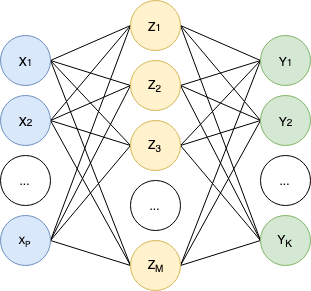
\includegraphics[width=0.6\textwidth]{images/nn_struct.png}
    \caption{Basic Multilayer Perceptron Schema}
    \label{fig:mlp-struc}
\end{figure}

The neural network has unknown parameters, called weights. For each connection between two nodes exists one weight. The set of all weights is denoted with $\Theta$. To generate these weights, the model is trained with a labelled training set. In each iteration, the error rate of the weights $R(\Theta)$ is being minimized using gradient decent, in this case called back-propagation. For classification, either the squared error or the deviance is used for the error function. \cite{hastie2005elements}

\begin{align}
    R(\Theta)=-\sum_{i=1}^N\sum_{k=1}^K y_{ik} \log f_k(x_i)
\end{align}{}

For the classification of the transportation mode, 27 features are generated. Thus, the Multilayer Perceptron classifier has 27 input nodes. The trained model can classify the two transportation modes walk and car. Thus, the classifier has two output layer nodes, one for each class to predict. 


\subsubsection{XGBoost}
XGBoost is a scalable tree boosting system. Since its release, it is successfully used in a number of machine learning competitions. Its success is mainly caused by its scalability. The scalability is due to a number of ''important systems and algorithmic optimizations''. Namely, these include a novel tree learning algorithm that can handle sparse data and also the introduction of approximate tree learning in its system. Due to this changes, the XGBoost ''runs more than ten times faster than existing popular solutions on a single machine''.  \cite{chen2016xgboost}

The basic algorithm of XGBoost is similar to other gradient boosting tree ensemble systems (Source Code \ref{code:xgboost}). The system iteratively tries to find the best decision tree for the given data, adds the created decision tree to a set of decision trees and increases the importance of the misclassified examples. In the following iteration, the system tries to find again the best decision tree, but due to the increased importance of the previously misclassified examples, these examples are more strongly considered. The algorithm stops if the maximum of allowed trees is generated. To classify an entry with the generated model, the entry is classified by each of the generated trees and their results are combined. \cite{chen2016xgboost}

\begin{lstlisting}[style=py, caption={Pseudocode: Basic XGBoost}, label={code:xgboost}]
def xgboostClassifyer(data, labels, maxTrees):
    i <- 0
    trees <- Array()
    while(i < maxTrees):
        decTree <- findBestDecisionTree(data, labels)
        trees.apped(decTree)
        increaseImportanceOfMissclassifiedData(decTree, data, label)
        i <- i + 1
    
    return trees
\end{lstlisting}

To generate the individual decision trees, several splits need to be chosen. The possible splits can be evaluated by a loss function. In XGBoost, this loss function is based on the difference between the prediction and target values of a split, as well as on the complexity of the model. The exact greedy algorithm is powerful in finding the next optimal split because it iterates over all possible next splits. The downside of the algorithm is that its performance suffers if the given data does not fits completely into the memory. To enable an efficient computation in this case, XGBoost implements an approximation algorithm for the split finding. \cite{chen2016xgboost}

The approximate algorithm for split finding (Source Code: \ref{code:xgboost_approx}) proposes splits for a percentile of each of the m features. The continuous features are sorted into buckets splits based on the generated candidate splits. The best solution among the proposed ones is aggregated. To calculate the score for each split, the algorithm uses the loss function of XGBoost, which is represented by the first and second order gradient statistics $g_j \in G$ and $h_j \in H$. 

\begin{lstlisting}[style=py, caption={Pseudocode: XGBoost - Approximate Algorithm for Split Finding \cite{chen2016xgboost} }, label={code:xgboost_approx}]
def approxSplitFinding():
    
    for k = 1 to m:
        Propose Splits S_k = {s_k1, S_k2, ... s_kl} by percentiles on feature k
    
    for k = 1 to m:
        G_kv <- all g_j, with s_kv >= x_jk > s_k,v-1
        H_kv <- all h_j, with s_kv >= x_jk > s_k,v-1
    
    return split with best score based on G and H
\end{lstlisting}








